\begin{figure}[htp]
    \centering
    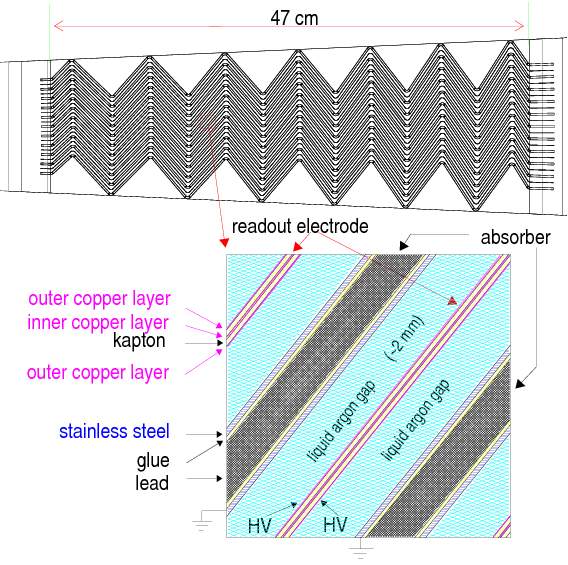
\includegraphics[width=0.5\textwidth]{figures/atlas/atlas_larg_module_accordion.png}
    \caption{Schematic for the accordion geometry (upper) of the LAr module, shown in a plane transverse to the LHC\@. Additionally, the layout of the readout electronics (bottom) is depicted, showing the liquid argon gaps and lead absorbers. This depicts the sampling architecture of the calorimeter nicely. Taken from~\cite{atlas_calorimeter_module_accordion}}\label{fig:atlas_calorimeter_accordion}
\end{figure}

The ECal is the inner most layer of the calorimeter system, surrounding the entire ID\@. As mentioned in the previous section, the ECal is a LAr based calorimeter where the active material is liquid argon and the passive absorbers are lead plates. Lead absorbers are chosen due to the high atomic number of the material resulting in a small $X_0$. The barrel region ($|\eta| < 1.475$) consists of two half barrels centered around the beam axis, with each half barrel consisting of 16 modules. The half barrels are separated from one another at $z = 0$ with a 4 mm gap. Each end-cap consists of two co-axial wheels, that are divided into eight modules, and cover the region $1.375 < |\eta| < 3.2$. Between the IP and calorimeter, there is approximately 1.7 \radlength, so to account for possible energy loss by electrons and photons a liquid-argon pre-sampler with resolution $\Delta\varphi \times \Delta\eta = 0.1 \times 0.025$ is placed in front of calorimeters in the range $|\eta| < 1.8$, allowing for an improved energy measurement. In the barrel and end-caps of the ECal, the lead absorbers and electrodes are accordion in shape, allowing for full coverage in $\varphi$. This accordion geometry, as well as the alternating pattern of liquid argon and lead, is seen in figure.~\ref{fig:atlas_calorimeter_accordion}. Overall, the ECal has a total of 180,000 readout channels. 

A LAr module consists of three different layers, with increasing granularity as distance from the IP increases\@. The first of these layers is the strip cells which have a resolution of $\Delta\varphi \times \Delta\eta = 0.1 \times 0.0031$, and extends for 4.3 \radlength{} before the second layer. The second layer consists of square cells with a resolution of $\Delta\varphi \times \Delta\eta = 0.025 \times 0.025$, and extends for at least 16.0 \radlength{} before reaching the third layer. This is the primary energy-depositing layer where the majority of the EM shower is absorbed. The third layer consists of coarser cells with a resolution of $\Delta\varphi \times \Delta\eta = 0.025 \times 0.05$, spanning approximately 2 \radlength. It is important to note that these \radlength{} correspond to $\eta = 0$ but differ depending on barrel $\eta$. Additionally, the third layer consists of even larger cells with a resolution of $\Delta\varphi \times \Delta\eta = 0.1 \times 0.1$, known as ``Trigger Towers'' (TTs), which were used in the Level-1 (L1) trigger system during the first two runs. For Run 3, the TT's are replaced\footnote{Technically, the TT's were not replaced but were supplemented with another technology that was meant to replace them eventually. The TT's were finally turned off in the middle of data taking in 2024.} with the new SuperCells that provide a more granular resolution. A comparison between the TT's and SuperCells can be seen in Figure~\ref{fig:atlas_super_cells}. Unlike the TT's, the SuperCells consists of four layers of varying granularity. The first layer (Layer 0), corresponding to the pre-sampler, has the same granularity as TT's of $\Delta\varphi \times \Delta\eta = 0.1 \times 0.1$. Layers 1 and 2 have a granularity as small as $\Delta\varphi \times \Delta\eta = 0.025 \times 0.1$, and the final layer returns to $\Delta\varphi \times \Delta\eta = 0.1 \times 0.1$. These changes allow for improved trigger algorithms, and provide a better definition of energy showers in the calorimeter. The trigger system will be discussed in more detail in Section~\ref{sec:atlas_trigger}. A sketch of a barrel module with the different layers can be seen in Figure~\ref{fig:atlas_calorimeter_module}.

\begin{figure}[htp]
    \centering
    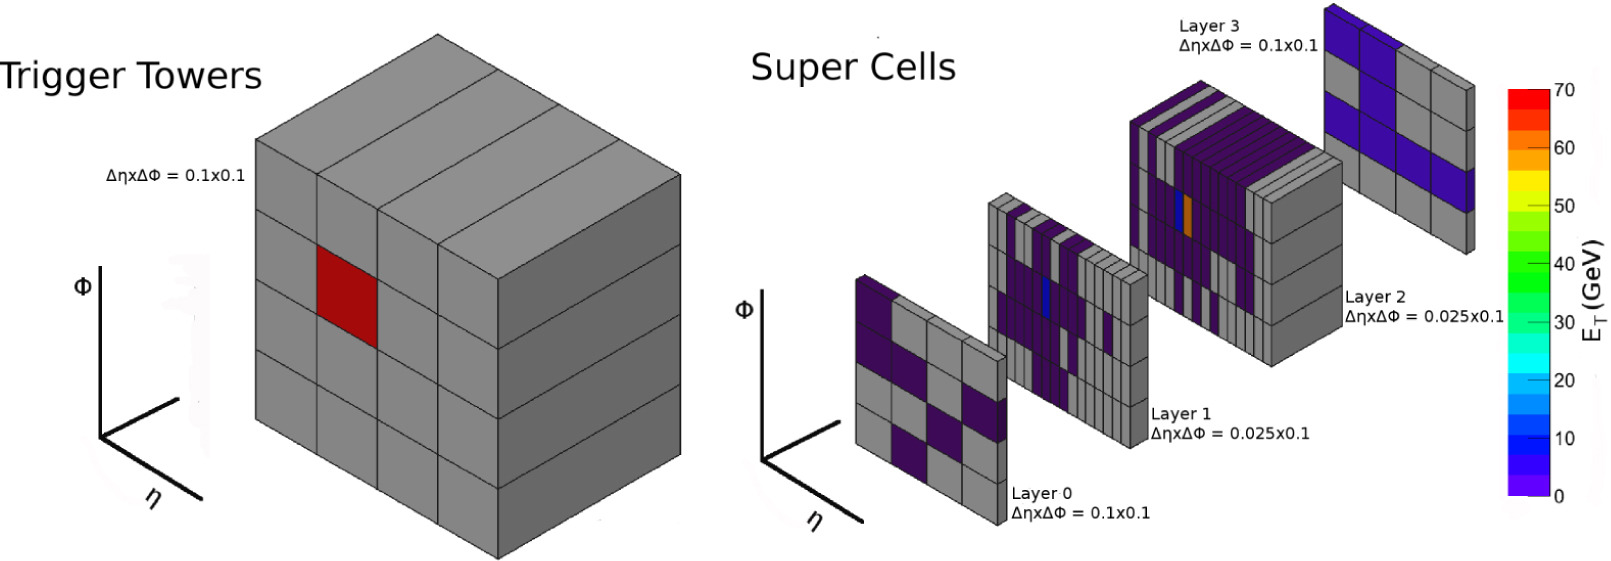
\includegraphics[width=0.8\textwidth]{figures/atlas/atlas_calorimeter_tt_to_supercell.jpg}
    \caption{A schematic comparison between a TT (left) and a SuperCell (right). The TT has a fixed granularity while the SuperCell has varying granularity allowing for more complex trigger algorithms. Taken from~\cite{atlas_calorimeter_supercell}}\label{fig:atlas_super_cells}
\end{figure}

\begin{figure}[htp]
    \centering
    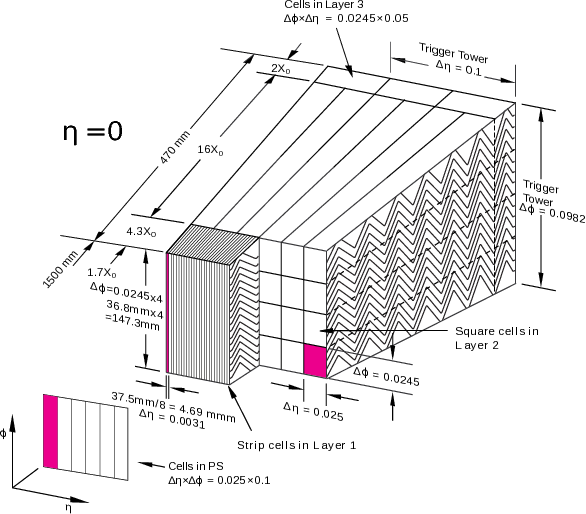
\includegraphics[width=0.7\textwidth]{figures/atlas/atlas_lar_module_cells.png}
    \caption{A sketch of a barrel module with its three different layers. The first layer consists of very granular strip cells, the second layer consists of square cells, and the third layer consists of slightly larger cells then the second layer. Taken from~\cite{atlas_calorimeter_module_accordion}}\label{fig:atlas_calorimeter_module}
\end{figure}

